\documentclass[a4paper, 12pt]{article} % Uses article class in A4 format

%----------------------------------------------------------------------------------------
%	FORMATTING
%----------------------------------------------------------------------------------------

\addtolength{\hoffset}{-2.25cm}
\addtolength{\textwidth}{4.5cm}
\addtolength{\voffset}{-3.25cm}
\addtolength{\textheight}{5cm}
\setlength{\parskip}{0pt}
\setlength{\parindent}{0in}

%----------------------------------------------------------------------------------------
%	PACKAGES AND OTHER DOCUMENT CONFIGURATIONS
%----------------------------------------------------------------------------------------

\usepackage{tabularx}
\usepackage{diagbox}
\usepackage{charter} % Use the Charter font
\usepackage[utf8]{inputenc} % Use UTF-8 encoding
\usepackage{microtype} % Slightly tweak font spacing for aesthetics

\usepackage[english]{babel} % Language hyphenation and typographical rules

\usepackage{tabularx}
\usepackage{mathrsfs}
\usepackage{amsthm, amsmath, amssymb} % Mathematical typesetting
\usepackage{float} % Improved interface for floating objects
\usepackage[final, colorlinks = true, 
linkcolor = black, 
citecolor = black]{hyperref} % For hyperlinks in the PDF
\usepackage{graphicx, multicol} % Enhanced support for graphics
\usepackage{color}
\usepackage{xcolor} % Driver-independent color extensions
\usepackage{marvosym, wasysym} % More symbols
\usepackage{rotating} % Rotation tools
\usepackage{censor} % Facilities for controlling restricted text
\usepackage{listings, lstautogobble} % Environment for non-formatted code
\usepackage{pseudocode} % Environment for specifying algorithms in a natural way
\usepackage{algorithm}
\usepackage{algpseudocode}
\renewcommand{\algorithmicrequire}{\textbf{Input:}}
\renewcommand{\algorithmicensure}{\textbf{Output:}}
\renewcommand{\algorithmicreturn}{\State \textbf{Return}}
\usepackage{booktabs} % Enhances quality of tables

\usepackage{cases}
\usepackage{bookmark}

\usepackage{tikz-qtree} % Easy tree drawing tool
\tikzset{every tree node/.style={align=center,anchor=north},
	level distance=2cm} % Configuration for q-trees

\usepackage[backend=biber,style=numeric,
sorting=nyt]{biblatex} % Complete reimplementation of bibliographic facilities

\usepackage{csquotes} % Context sensitive quotation facilities

\usepackage[yyyymmdd]{datetime} % Uses YEAR-MONTH-DAY format for dates
\renewcommand{\dateseparator}{-} % Sets dateseparator to '-'

\usepackage{fancyhdr} % Headers and footers
\pagestyle{fancy} % All pages have headers and footers
\fancyhead{}\renewcommand{\headrulewidth}{0pt} % Blank out the default header
\fancyfoot[L]{} % Custom footer text
\fancyfoot[C]{} % Custom footer text
\fancyfoot[R]{\thepage} % Custom footer text

\newcommand{\note}[1]{\marginpar{\scriptsize \textcolor{red}{#1}}} % Enables comments in red on margin

\usepackage{fontspec}
\setmonofont{Consolas}
\definecolor{codegreen}{rgb}{0,0.6,0}
\definecolor{codegray}{rgb}{0.5,0.5,0.5}
\definecolor{codemauve}{rgb}{0.58,0,0.82}

\lstset{ %
	language=python,                % choose the language of the code
	basicstyle=\footnotesize\ttfamily,       % the size of the fonts that are used for the code
	numbers=left,                   % where to put the line-numbers
	numberstyle=\tiny\color{codegray},      % the size of the fonts that are used for the line-numbers
	stepnumber=1,                   % the step between two line-numbers. If it is 1 each line will be numbered
	numbersep=5pt,                  % how far the line-numbers are from the code
	backgroundcolor=\color{white},  % choose the background color. You must add \usepackage{color}
	showspaces=false,               % show spaces adding particular underscores
	showstringspaces=false,         % underline spaces within strings
	showtabs=false,                 % show tabs within strings adding particular underscores
	frame=single,                   % adds a frame around the code
	tabsize=4,                      % sets default tabsize to 4 spaces  
	captionpos=b,                   % sets the caption-position to bottom
	breaklines=true,                % sets automatic line breaking
	breakatwhitespace=false,        % sets if automatic breaks should only happen at whitespace
	escapeinside={\%*}{*)},
	commentstyle=\color{codegreen},
	keywordstyle=\bfseries\color{magenta},
	stringstyle=\color{red},
	identifierstyle=\color{codemauve},
	keepspaces=true
	autogobble=true
}

%----------------------------------------------------------------------------------------

\begin{document}
	
	%----------------------------------------------------------------------------------------
	%	TITLE SECTION
	%----------------------------------------------------------------------------------------
	
	\title{Template} % Article title
	\fancyhead[C]{}
	\hrule \medskip % Upper rule
	\begin{minipage}{0.295\textwidth} % Left side of title section
		\raggedright
		DATA130008\\ % Your course code
		\footnotesize % Authors text size
		\hfill\\
		Introduction to Artificial Intelligence\\ % Your course name
	\end{minipage}
	\begin{minipage}{0.4\textwidth} % Center of title section
		\centering
		\large % Title text size
		Final Report\\ % Assignment title and number
		\normalsize % Subtitle text size
	\end{minipage}
	\begin{minipage}{0.295\textwidth} % Right side of title section
		\raggedleft
		BoYuan Yao 19307110202\\ % Your name
		LeiRu Long 19307130350
		\footnotesize % Email text size
		\hfill\\
		\today\\ % Date
	\end{minipage}
	\medskip\hrule % Lower rule
	\bigskip
	
\paragraph{Abstract}
	In the last two checkpoints, we have already implemented Alpha-Beta Pruning algorithm and MCTS algorithm on Gomoku AI. After learning some basic concept of reinforcement learning, we constructed a prototype AI using the idea of QLearning. We also improved our Alpha-Beta Pruning AI for better performance.
		
	\begin{multicols}{2}
		[
		\section{Introduction}
		]
		Reinforcement learning has become a hot topic in recent years. Agent could learn the policy of given environment by interacting with the given environment. With the aids of neural network, reinforcement learning could achieve better performance (e.g. AlphaGo Zero). We have learned some Model-Based and Model-Free learning policies on class. So we implemented a QLearning-based AI to enhance our understanding of the lectures.
		
		Moreover, as we learned after class, there are also some advanced methods of tranditional searching policy. The PVS (Principal Variation Search) is a good way to promote the pruning ability of Alpha-Beta Pruning. We also find several ways to shorten the searching time.
		
		The organization of the report is as follows. In the next section we will give a brief description of QLearning and our implementation of reinforcement learning checkpoint. In the third section, we will introduce the improvement of our Alpha-Beta Pruning Algorithm. We will plot our experimental result in the following section and in the last one, we will conclude what we learned in the Gomoku project and some more future work.
		
		
	\end{multicols}
	
	\bigskip
	
	%------------------------------------------------
	
	\begin{multicols}{2}
		[
		\section{Q-Learning AI}
		]
		\subsection{Q-Learning}
		
		The key idea of Q-Learning is, maintaining the state-action Q estimates and use the value of the best future action for bootstrap update. It's a famous off policy startegy, with the following iteratiom
		
		\begin{equation*}
			\begin{split}
				& Q(s_t, a_t)  = Q(s_t, a_t) + \alpha \delta_t \\
				& \delta_t  = r_t + \gamma \max\limits_{a'}Q(s_{t + 1}, a') - Q(s_t, a_t)
			\end{split}
		\end{equation*}
	
		Where $\delta_t$ is known as TD error. This off-policy learning strategy really fit our target, as training the Gomoku AI is costly (though mush easier than Go) and, we need historical data from old polices (i.e. the information of former training derive by the old agent).
		
		\subsection{Sigmoid}
		
		Sigmoid function is a famous function used in neural network. As we know, without sigmoid function, neural network just contain several matrix operations, which means it could only represent the linear model. But with the sigmoid function, neural network gains the ability to represent nonlinear information, which is important beacuase most of the real-life models involve a lot of nonlinear relations. Moreover, sigmoid function is a good transformation of value in interval $(-\infty, +\infty)$ to interval $(0, 1)$, which provides a good way for evaluation-to-win-rate transform. It has the following form
		
		
		\begin{equation*}
			S(t) = \frac{1}{1 + e^{-t}}
		\end{equation*}
	
		We could attain a simple property, that $S'(t) = S(t)(1 - S(t))$, meaning that we could easily attain the gradient of function $S$ at $t$ just using $S(t)$.
		
		\subsection{Q-value}
		
		With the idea of sigmoid function, we could transform our evaluation to a winning rate. So in our RL AI, we compute the Q-value with the following equation
		
		\begin{equation*}
			\text{Q-value} = \frac{1}{1 + e^{-\beta s(f)}}
		\end{equation*}
	
		Where $s(f)$ stands for the score of the given features, and $\beta$ stands for a shrink coefficient to avoid the extremely small difference of the value of sigmoid function with efficiently large (w.r.t absolute value) of $x$.
		
		\subsection{Feature Extractor}
		
		We inherent the feature of the last Alpha-Beta Pruning AI, i.e. scanning the four directions of a empty point and extract the pattern inside it. With all these features, our AI could return a Q-value for each action.
		 
		\subsection{Root Search}
		We inherent the tree search process in MCTS, using the following tree policy
		
		\begin{algorithm}[H]
			\caption{Tree Policy}
			\begin{algorithmic}[1]
				\Require root state $s_0$
				\Ensure selected son of root state $candidate$
				\Return $candidate$ with biggest Q-value
			\end{algorithmic}
		\end{algorithm}
	
		Notice that if a $candidate$ hasn't been explored, the Q-value of this son node is 1, so that every active son of the current root state will be explored.
		
		\subsection{Feedback}
		
		Adopting the feedback structure in Project-3, the feedback module deliverying the impact of reward at leaf node (as we attain the outcome of the game) all the way back to root node. As we using sigmoid, the iteration is as follows
		
		\begin{equation*}
			weight(f_{t + 1}) = weight(f_t) + \alpha \delta_t v \beta (1 - Q)Q
		\end{equation*}
		
		Where the $\delta_t$ is the TD error in 2.1, $\alpha$ is the learning rate, $\beta$ is a shrink coefficient to avoid the extremely small difference of the value of sigmoid function with efficiently large $x$, and $v$ is the number of the given feature $f$.
		
		\subsection{Simulation}
		
		Inherenting the simulation in our MCTS AI, the simulation policy involves $\epsilon$-greedy to balance the exploration and exploitation and generate enough data for learning.
		
		\subsection{Training Policy}
		
		We apply the following training policy
		
		\begin{algorithm}[H]
			\caption{Training policy}
			\begin{algorithmic}[1]
				\Require initial policy
				\Ensure new policy
				\State new policy $\gets$ initial policy
				\While{Doesn't meet stopping criteria}
					\While{new policy could not beat initial policy}
						\State generate data using self-play method with initial policy
						\State update new policy with the data
					\EndWhile
					\State initial policy $\gets$ new policy
					\State Check stopping criteria
				\EndWhile
			\end{algorithmic}
		\end{algorithm}
	
		The idea is natural selection, killing the old AI with old policy ,updating the fighting policy of data generation group and pushing the AI to find the stronger policy.
	\end{multicols}
	
	\newpage
	
	\begin{multicols}{2}
		[
		\section{Improvement of Alpha-Beta Pruning AI}
		The original Alpha-Beta pruning stratgy could not meet the standard of high peformance searching, with the help of PVS, iterating deepening search, moves pruning, mapping technics we could achieve better performance. The basic idea of our work is based on the AI WINE.
		]

		\subsection{PVS}
		
		PVS (Principal Variation Search) is an improved version of origin Alpha-Beta algorithm. As we learned in Alpha-Beta Pruning, we know that the meaning of "Alpha-Beta" is, in fact, a window for searching. As the searching proceeding, the window will shrink and we will get an exact value for root node. In fact we could divide searching nodes into the following three kinds:
		
		\begin{itemize}
			\item Alpha node. In alpha node, every branch will return a value lower than current Alpha.
			\item Beta node. In beta node, at least one branch will return a value bigger than Beta.
			\item PV node. In exact node, every branch will return a value between interval $(Alpha, Beta)$
		\end{itemize}
	
		We could see that Alpha-Beta Pruning will prune the subtree with root falls into the first two kind. But for PV node, it takes more time for searching beacuse we can not apply any kinds of pruning. So our wish is, we could have a window with zero width, i.e. we have the "midpoint" of all the son nodes, so that all the nodes belongs to Alpha node or Beta node, given an exact value for root node with high efficiency.
		
		So in implementation, we suppose we have already found that sweat point, and deploy an Alpha-Beta search of zero-width window to prove our assumption. If we get a value satisfies $val \leq alpha$, then we have found the best evaluation $alpha$, otherwise our assumption fail, we need to do one step Alpha-Beta Pruning with normal-width searching window. 
		
		Though we might waste sometime on the attempt of zero-width window searching, we gain bigger edge when the assumption works, easily promoting the pruning ability of the AI.
		
		\begin{algorithm}[H]
			\caption{Alpha-Beta pruning with PVS}
			\begin{algorithmic}[1]
				\Require $\alpha, \beta, root$
				\Ensure Exact value for $root$ $val$
				\While{$root$ has kids}
					\If{not the first kid and $\alpha + 1 < \beta$}
						\State $val \gets -AlphaBeta(-\alpha - 1, -\alpha)$
						\If{$val$ in interval $(\alpha, \beta)$}
							\State $val \gets -AlphaBeta(-\beta, -\alpha)$
						\EndIf
					\EndIf
					\State Update $alpha$ if needed
				\EndWhile
				\Return $val$
			\end{algorithmic}
		\end{algorithm}
		
		\subsection{Iterating deepening search}
		
		Considering the limited time we have on the Gomoku game, iterating deepening search is a great method for time management. As we can not find the whole story of one game just for one Alpha-Beta search (explonential work !!), we just iteratively deepening the searching depth so that we could find better answer if we have time for more searching layers, and find a proximal solution without violating the time limits if we don't have that much time. To maximize the power of iterating deepening search, we need the help of zobrist hash.
		
		\subsection{Zobrist Hash}
		
		\begin{figure}[H]
			\centering
			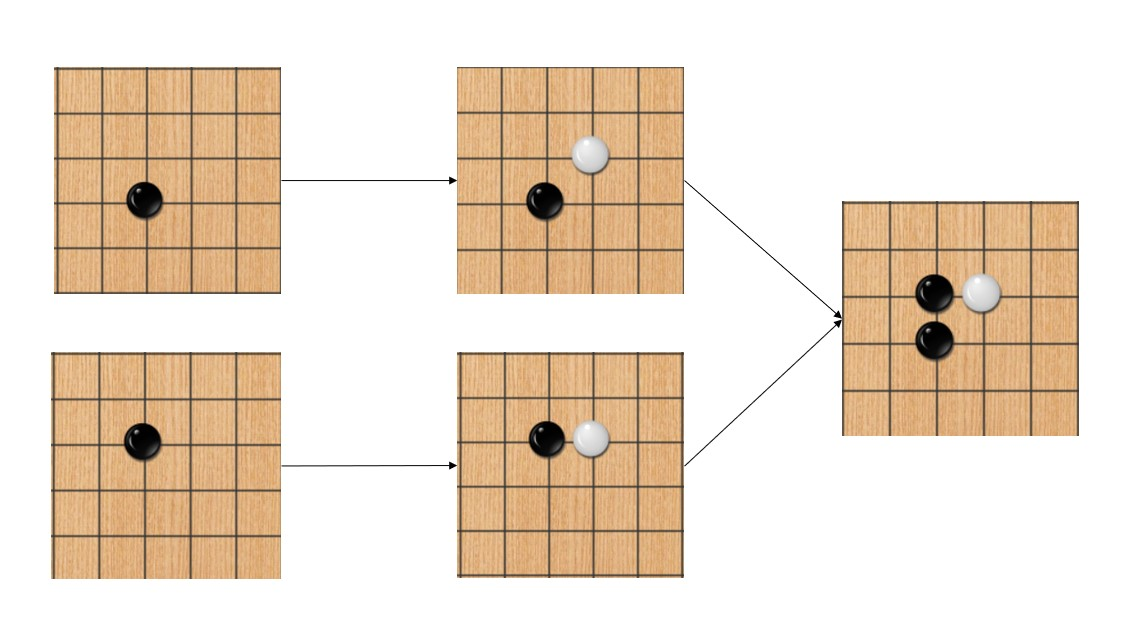
\includegraphics[scale=0.35]{zobristhash.jpg}
			\caption{Why using zobrist hash}
		\end{figure}
	
		As we conclude in the first report, zobrist hash is a good way to store all the expanded move. But due to the bad data structure in our last AI, it is risky to use zobrist hash and it consume a lot of time. This time we reform our AI and apply the zobrist hash to our program. Not only did we apply the zobrist hash on move update, but we also deployed it on the Alpha-Beta search process, storing the some key information of each node, which could be a great boosting for the performance of iterating deepening search.
		
		In our implementation, when the AI expand next move, it will first searching the $pvsTable$, to search for the best move recorded during the Alpha-Beta process, otherwise it will generate all the moves possible. We will record the node information in the $hashtable$, and whenever the Alpha-Beta process or iterating deepening search use the recorded node information (with depth not less than current depth), it could reuse it to avoid searching. Which means the cost of iterating deepening search will be minimized as it reuse the information of former searched layers.
		
		\subsection{Moves Pruning}
		When generating the moves in our last Alpha-Beta AI, we simply generate all the moves and sort them in descending order. And for the move which is realy important, we just using the function $seek\_must$ at the very begining to find the winning moves or defending moves to avoid losing the game. But it is really short-sighted. Therefore, in this AI, we applyed moves pruning on each moves generation, it works as follows
		
		\begin{algorithm}[H]
			\caption{Moves pruning}
			\begin{algorithmic}[1]
				\Require moves list $cand$
				\Ensure pruned move list $cand$
				\If{best move could form at least FLEX4}
					\Return the very first move of $cand$
				\ElsIf{The opponents has FLEX3}
					\State Find the oppnents move which could form FLEX4
					\State Find the move for both sides which could form BLOCK4
					\Return the above moves
				\EndIf
				\Return origin $cand$
			\end{algorithmic}
		\end{algorithm}
	
		Where the renewed pattern table is as follows:
		
		\begin{table}[H]
			\setlength\tabcolsep{3pt}
			\begin{center}
				\scalebox{0.9}{
					\begin{tabularx}{8cm}{ccc}
						\toprule
						\textbf{Pattern Type} & \textbf{Definition} & \textbf{Value}\\
						\midrule
						WIN
						&\begin{minipage}[b]{0.3\columnwidth}
							\centering
							\raisebox{-.5\height}{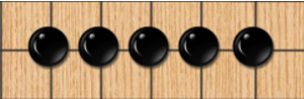
\includegraphics[width=\linewidth]{five.png}}
						\end{minipage}
						& 1200 \\
						\midrule
						FLEX4 & \begin{minipage}[b]{ 0.3\columnwidth}
							\centering
							\raisebox{-.5\height}{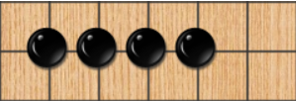
\includegraphics[width=\linewidth]{4.png}}
						\end{minipage} & 800 \\
						\midrule
						BLOCK4 & \begin{minipage}[b]{ 0.3\columnwidth}
							\centering
							\raisebox{-.5\height}{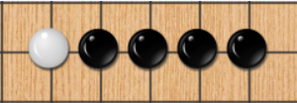
\includegraphics[width=\linewidth]{b4.png}}
						\end{minipage} & 144 \\
						\midrule
						FLEX3 & \begin{minipage}[b]{ 0.3\columnwidth}
							\centering
							\raisebox{-.5\height}{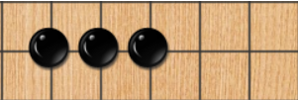
\includegraphics[width=\linewidth]{3.png}}
						\end{minipage} & 96 \\
						\midrule
						BLOCK3 & \begin{minipage}[b]{ 0.3\columnwidth}
							\centering
							\raisebox{-.5\height}{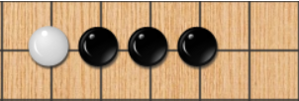
\includegraphics[width=\linewidth]{b3.png}}
						\end{minipage} & 18 \\
						\midrule
						FLEX2 &\begin{minipage}[b]{ 0.3\columnwidth}
							\centering
							\raisebox{-.5\height}{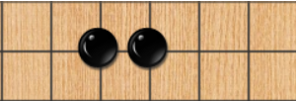
\includegraphics[width=\linewidth]{2.png}}
						\end{minipage} & 12 \\
						\midrule
						BLOCK2 & \begin{minipage}[b]{ 0.3\columnwidth}
							\centering
							\raisebox{-.5\height}{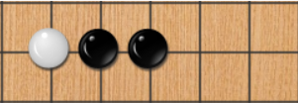
\includegraphics[width=\linewidth]{b2.png}}
						\end{minipage} & 2 \\
						\bottomrule
					\end{tabularx}
				}
				\caption{Score For Each Pattern}
				\label{tab:table1}
			\end{center}
		\end{table}
	
	\subsection{Mapping technics}
	
		In our first Alpha-Beta Pruning AI, the scanning process occurs each time we update the score of the table. With a lot of optimization, the updating process did cost less time than before. However, there are better solutions for the evaluating and updating process. When initialization the basic structure, we simply construct a table for each pattern, and to seek for pattern for a certain point and in a certain direction, all we need to do is derive a key using the information of the neighbors. Here is a simple example of how we manage to do it.
		
		\begin{figure}[H]
			\centering
			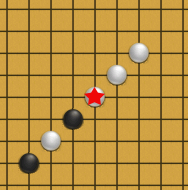
\includegraphics[scale=1.0]{XORexample.png}
			\caption{Example for mapping technics}
		\end{figure}
	
		To evaluate the point with red star in the reverse diagonal direction, we could derive a key using XOR operation. In this case, assuming in the AI module we have 0 stands for white piece ,1 stands for black piece and 2 stands for empty place, then the key (in one direction) is
		
		\begin{eqnarray*}
			\begin{split}
				key = & 2 \^{} (1 << 2) \^{} (0 << 4) \^{} (1 << 6) \^{} \\
				& (0 << 8) \^{} (0 << 10) \^{} (2 << 12) \^{} (2 << 14) 
			\end{split}
		\end{eqnarray*}
	
		Where $\^{}$ stands for bit XOR and $<<$ stands for the shift operation.
		
		And with the given key, we could check the pattern in the initialized structure $pattern\_table$ in my AI. Which is much faster than before, avoiding all the scanning operation in between the searching process, but finishing all of them at a table at initialization, saving tons of time. Moreover, we even stores the pattern value for various of cases in the structure $pval\_table$, which furture optimize the performance of the AI.
		
	\end{multicols}

	\bigskip
	
	\begin{multicols}{2}
		[
		\section{Experimental Result}
		]
		
		\subsection{Q-Learning Result}
		
		The initial weights and the learned whights (4000 rounds of learning) are as follows:
		
		\begin{center}
			\begin{tabular}{|c|c|c|}
				\hline$-$ & initial & learned\\
				\hline \hline WIN & $600$ & $599.9297$\\
				\hline \hline FLEX4 & $400$ & $399.5267$\\
				\hline \hline BLOCK4 & $150$ & $ 146.6131$\\
				\hline \hline FLEX3 & $70$ & $64.4071$\\
				\hline \hline BLOCK3 & $20$ & $16.7302$\\
				\hline \hline FLEX2 & $10$ & $1.1991$\\
				\hline \hline BLOCK2 & $2$ & $-4.4021$\\
				\hline \hline FLEX1 & $10$ & $-22.9923$\\
				\hline \hline BLOCK1 & $0$ & $-17.2641$\\
				\hline
			\end{tabular}
		\end{center}
		
		With the learned policy, we test the agent on our computer with some AIs, and here is the result
		
		\begin{center}
			\begin{tabular}{|c|c|}
				\hline$-$ & abpruning\\
				\hline \hline pisq7 & $2:10$ \\
				\hline \hline valkyrie & $8:4$ \\
				\hline \hline mushroom & $10: 2$ \\
				\hline \hline fiverow & $12: 0$ \\
				\hline
			\end{tabular}
		\end{center}
		
		The learned policy works pretty well.
		
		\subsection{Alpha-Beta Pruning Result}
		Setting the maximum searching depth 8 and maximum branch of each layer 8, we attain the following result on ftp
		
		\begin{tabular}{|c|c|c|c|}
			\hline$-$ & abpruning & & abpruning\\
			\hline \hline pisq7 & $12: 0$ & Yixin2018 & $1: 11$ \\
			\hline \hline Noesis & $9: 3$ & Eulring & $3: 9$ \\
			\hline \hline Wine18 & $1: 11$ & valkyrie & $12: 0$\\
			\hline \hline Sparkle & $9: 3$ & fiverow & $12: 0$ \\
			\hline \hline zetor2017 & $7: 5$ & PureRocky & $12: 0$ \\
			\hline \hline pela & $1: 11$ & mushroom & $12: 0$ \\
			\hline
		\end{tabular}
		
		The final Elo rating for our AI is 1666.
	\end{multicols}

	\bigskip
	
	\begin{multicols}{2}
		[
		\section{Conclusion and Future Work}
		]
		\begin{figure}[H]
			\centering
			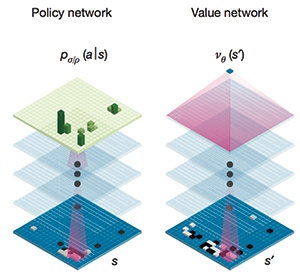
\includegraphics[scale=0.5]{Network.jpg}
			\caption{AlphaGo Networks}
		\end{figure}
		With weeks of hard work, our AI really improved a lot. But with the limitation of background knowledge and time (also the performance of python is not that good), there are still a lot of improvements could be done. For tranditional method, we are lack of the time to implement a powerful checkmate module, as we found that the last checkmate in our AI has some problems that could even make the result worse. And the combination of checkmate and Alpha-Beta pruning is also a field worth trying, as checkmate is much faster than Alpha-Beta pruning (also more accurate).
		
		For RL, as we searching online, we found a lot of AI using the deep learning technics to enhance there ability to express the variation on board. There are usually plenty of networks for different phases, e.g in AlphaGo, they have a policy network and value network to give policy and evaluate the win rate. With limited time and space constrain (we could not use numpy due to the 20M constraint), it is really hard and inefficient to construct the neural network and training them until they could work.
		
	\end{multicols}

	\section{Acknowledgement}
		Thanks a lot for TA's patient tutorials, and in time reply when we met some problem runnning AI on the ftp folder.
		
	\begin{thebibliography}{99}
		\bibitem{ref1} Zhentao Tang, Zhao, D., Kun Shao, Le Lv. (2016). ADP with MCTS algorithm for Gomoku. 2016 IEEE Symposium Series on Computational Intelligence (SSCI).
		\bibitem{ref2} C. B. Browne, E. Powley, D. Whitehouse, S. M. Lucas, P. I. Cowling, P. Rohlfshagen, S. Tavener, D. Perez, S. Samothrakis, and S. Colton, "A Survey of Monte Carlo Tree Search Methods," IEEE Transactions on Computational Intelligence and AI in Games, vol. 4, pp. 1-43, 2012.
		\bibitem{ref3} Chang, H.S., M.C. Fu, J. Hu, and S.I. Marcus. 2016. “Google Deep Mind’s AlphaGo”. OR/MS Today.
		\bibitem{ref4}L. Allis, H. Herik, and M. Huntjens. Go-moku and
		threat-space search. Computational Intelligence, 12, 10 1994.
		\bibitem{ref5}Pearl, Judea. "The solution for the branching factor of the alpha-beta pruning algorithm and its optimality." Communications of the ACM 25.8 (1982): 559-564.
		\bibitem{ref6}Albert Zobrist (1970). A New Hashing Method with Application for Game Playing. Technical Report, Computer Science Department, The University of Wisconsin, Madison, WI, USA.
		\bibitem{ref7}J. Lawrence Carter, Mark N. Wegman (1977). Universal classes of hash functions. STOC'77
		\bibitem{ref8}Tony Marsland, Murray Campbell. Parallel Search of Strongly Ordered Game Trees. ACM Comput. Surv. 1982, 14(4): 533-551.
		\bibitem{ref8} Lorenzo Piazzo ,Michele Scarpiniti ,Enzo Baccarelli. Gomoku: analysis of the game and of the player Wine. CoRR. 2021, abs/2111.01016. 
	\end{thebibliography}
	%----------------------------------------------------------------------------------------
	%	REFERENCE LIST
	%----------------------------------------------------------------------------------------
	
	% \cite{Bird2014}
	% \printbibliography
	
	%----------------------------------------------------------------------------------------
	
\end{document}
